%%%%%%%%%%%%%%%%%%%%%%%%%%%%%%%%%%%%%%%%%%%%%%%%%%%%%%%%%%%
% EPFL report package, main thesis file
% Goal: provide formatting for theses and project reports
% Author: Mathias Payer <mathias.payer@epfl.ch>
%
% This work may be distributed and/or modified under the
% conditions of the LaTeX Project Public License, either version 1.3
% of this license or (at your option) any later version.
% The latest version of this license is in
%   http://www.latex-project.org/lppl.txt
%
%%%%%%%%%%%%%%%%%%%%%%%%%%%%%%%%%%%%%%%%%%%%%%%%%%%%%%%%%%%
\documentclass[a4paper,11pt,oneside]{report}
% Options: MScProject, 


\usepackage[MScProject]{EPFLreport}
\usepackage{xspace}
\usepackage{charter}
\usepackage{amsmath}
\usepackage{amsfonts}
\usepackage{mathtools}
\usepackage[ruled,vlined]{algorithm2e}
\microtypecontext{spacing=nonfrench}
\usepackage{csquotes}


\title{Stochastic variance reduced gradient methods for training Deep Neural Networks}
\author{Alexander Apostolov}
\supervisor{Dr. Tatjana Chavdarova}
\adviser{Prof. Dr. Martin Jaggi}


\begin{document}
\maketitle
%\makededication

\begin{abstract}

This project focuses on analyzing the effect of stochastic variance reduced gradient methods on training Deep Neural Networks (DNNs). This project mainly focuses on one stochastic variance reduced gradient methods, SVRG and gives some insights about another one, STORM. Despite their proved theoretical advantages and their relative straightforwardness, these methods remain unpopular because they are performing poorly on popular deep neural networks for reasons that are yet not theoretically proved.  

This project follows an empirical approach to improve our understanding  why variance reduction method fail to  perform well on DNNs. We show that these methods perform well on shallow neural networks and give insights on why we generally have worse results on deeper architectures. We also show that removing batch-normalization layers from deep neural networks tends to help stochastic variance reduced gradient methods when compared to other stochastic methods in the same setup.

\end{abstract}

\maketoc

%%%%%%%%%%%%%%%%%%%%%%
\chapter{Introduction}
%%%%%%%%%%%%%%%%%%%%%%

Optimization problems are a centerpiece of many machine learning tasks and choosing an appropriate optimization algorithm is a crucial step to get good results. Stochastic variance reduced gradient methods\footnote{Herein referred as \textit{Variance Reduced},  for short.} have been shown to theoretically have better convergence than stochastic gradient descent methods. However, they are not widely used as they seem to be outperformed on most standard deeper neural networks.  
These worst performances have been empirically described~\cite{Defazio2019} but there are no theoretical insights on the reasons for that.  

This project tries to build an empirical approach to improve our understanding on why variance reduction methods fail to perform well on DNNs. To do so we look at \textbf{Stochastic Variance Reduced Gradient} \textbf{(SVRG)}~\cite{NIPS2013_ac1dd209} and \textbf{STOchastic Recursive Momentum} \textbf{(STORM)}~\cite{Cutkosky2019storm}, two variance reduced methods and compare them on different architectures. We compare them with \textbf{Stochastic Gradient Descent (SGD)} and \textbf{Adam}~\cite{kingma2014adam}.  

We think that using batch-normalization layers in the neural network might be one of the reasons of the worse performance of variance reduced methods, so we perform different experiments using networks with and without these layers. Finally, we think that having better weight initialization can help in the cases when we are training on DNNs without batch-normalization layers, so we try to observe effects by using \textbf{MetaInit}~\cite{NEURIPS2019_876e8108}, an algorithm that helps finding weights before starting to train a model.


%%%%%%%%%%%%%%%%%%%%
\chapter{Related Works}
%%%%%%%%%%%%%%%%%%%%

In machine learning, the following optimization is often encountered.
Let $w$ denote the model parameters, and let $f_1, f_2, \dots, f_n$ be a sequence of vector functions $\mathbb{R}^d \mapsto \mathbb{R}$ where each $f_i(\cdot)$ is the loss on a single training data point.
The goal is to find a solution to the following ``finite-sum'' problem:
\begin{equation}\label{eq:minimzing_function}
    \min_w F(w),~~F(w)=\frac{1}{n}\sum_{i=1}^n f_i(w).
\end{equation}

There are many examples of such functions we need to minimize, they are often referred to as loss functions. When trying to do predictions in $\mathbb{R}$ using features very common ones are Mean Square Error (MSE), Mean Absolute Error (MAE). Given a dataset $S=\{(y_i, x_i)_{i=1\}^n}$ where $y_i \in \mathbb{R}$ and $x_i \in \mathbb{R^d}$ and a prediction function $p_w : \mathbb{R^d} \mapsto \mathbb{R}$ depending on some weights or parameters $w$, the Mean Square Error is defined as:
$$F_{MSE}(w) = \frac{1}{2n}\sum_{i=1}^n(y_i - p_w(x_i))^2$$
In the same setting, the Mean Absolute Error is defined as:
$$F_{MAE}(w) = \frac{1}{n}\sum_{i=1}^n\mathopen|y_i - p_w(x_i)\mathclose|$$
Another example of such loss functions we are trying to minimize in image segmentation tasks is the Jaccard Loss. Given some images where we want to detect some areas of interest (free rooftop areas for photovoltaic panels installations in satellite images, pedestrians on images from a car etc$\dots$) we can be given the set of correct labels $y_i \in \{0,1\}^{H \times W}$ for some images $x_i \in \mathbb{R}^{H \times W}$ of height $H$ and width $W$ and we wish to find a function $p_w$ which assigns a label 1 or 0 to each pixel to indicate weather it is in the area of interest or not: $p_w : \mathbb{R}^{H \times W} \mapsto \{0,1\}^{H \times W}$. Then the Jaccard loss is given by:
$$F_{Jaccard}(w) = \frac{1}{n}\sum_{i=1}^n \frac{p_w(x_i) \cap y_i}{p_w(x_i) \cup y_i}$$

A widely used and straightforward method to solve \autoref{eq:minimzing_function} is to use \textbf{Gradient Descent (GD)}. This method relies on the fact that the gradient of a function, $\nabla F(w^{(t)})$, points towards the steepest ascent direction, so one can use the opposite direction of the gradient to go towards a minimum of a function. This method is iterative, at each iteration $t=1,2, \dots T$ we calculate new weights for $F(w)$ by:
\begin{equation}\label{eq:GD}
    w^{(t)} = w^{(t-1)} - \eta_t \nabla F(w^{(t-1)}) \,,
\end{equation}
where $\eta_t$ is the learning rate at iteration $t$.
A problem with Gradient Descent is that each update step requires computing the gradient over the whole dataset. This can require a lot of computations, making this algorithm inefficient for some tasks. 

This drawback is why \textbf{Stochastic Gradient Descent (SGD)} has been widely adopted. Instead of computing the gradient over the whole dataset at each iteration, we an only use the gradient with respect to one datapoint. The algorithm is given by the following update rule. At each iteration $t=1,2 \dots T$, sample one datapoint $i_t \in \{1,\dots n\}$ uniformly at random:
\begin{equation}\label{eq:SGD}
    w^{(t)} = w^{(t-1)} -\eta_t \nabla f_{i_t}(w^{(t-1)})\,,
\end{equation}
where $\eta_t$ is the learning rate at iteration $t$.

This idea behind this trick is that it decreases the computational complexity of each iteration by a factor of $\theta(1/n)$ and one can show that in expectation the gradient in SGD is equal to the full gradient over the whole dataset:
\begin{equation}\label{eq:unbaisedSGD}
    \mathbb{E}[\nabla f_{i_t}(w)] = \nabla F(w)\,.
\end{equation}

A very similar method is the so called \textbf{Mini-batch SGD} where instead of choosing one datapoint $x_{i_t}$, we choose a subset $B_t$ of all the datapoints uniformly at random at each iteration and then use the following  rule. For each iteration $t = 1,2 \dots T$:
\begin{equation}\label{eq:minibatchSGD}
    w^{(t)} = w^{(t-1)} -\eta_t \frac{1}{\mathopen|B_t\mathclose|}\sum_{i \in B_t}\nabla f_{i}(w^{(t-1)})\,,
\end{equation}
where $\eta_t$ is the learning rate at iteration $t$.

Both Stochastic Gradient Descent and Mini-batch Stochastic Gradient Descent use an unbiased estimate of the gradient to have faster iterations, but using only a subset of the dataset \textbf{increases the variance} of the gradient estimates, which slows down convergence. There is thus a trade-off between fast per iteration computations and fast convergence. Variance reduced methods allow us to get a better deal from this trade-off by keeping fast per-iteration computations while maintaining a fast convergence.

In this project we will analyze two variance reduced algorithms: \textbf{Stochastic Variance Reduced Gradient} \textbf{(SVRG)}~\cite{NIPS2013_ac1dd209} and \textbf{STOchastic Recursive Momentum} \textbf{(STORM)}~\cite{Cutkosky2019storm}. 

SVRG is an iterative algorithm whose goal is to solve \autoref{eq:minimzing_function} by using elements of Stochastic Gradient Descent to ensure fast iterations in terms of computational complexity and Gradient Descent to get low variance. The main idea behind this algorithm presented by Rie Johnson and Tong Zhang in 2013 is that we do a snapshot $\Tilde{w}$ of the parameters every $m$ iterations and compute the gradient $\Tilde{\mu}$ over the whole dataset with respect to $\Tilde{w}$ to get an estimate of the true gradient. Similarly to SGD, we take a datapoint $x_{i_t}$(or more generally a mini-batch) uniformly at random at each iteration $t=1,2,\dots T$ and apply the following update rule:
\begin{equation}\label{eq:updateSVRG}
    w^{(t)} = w^{(t-1)} -\eta(\nabla f_{i_t}(w^{(t-1)}) - \nabla f_{i_t}(\Tilde{w}) + \Tilde{\mu})\,,
\end{equation}
where $\Tilde{w}$ is snapshot of $w$ taken when $\Tilde{\mu}$ is computed every $m$ iterations, and:
\begin{equation}\label{eq:snapshotGradientSVRG}
    \Tilde{\mu} = \nabla F(\Tilde{w}) = \frac{1}{n}\sum_{i=1}^n \nabla f_i(\Tilde{w})\,.
\end{equation}

The hyperparameter $m$ is usually in the order of a few epochs. The original paper suggests setting $m$ to $3$ or $5$ epochs for convex objectives and non-convex objectives such as Neural Networks respectively. 

An important thing to note is that $\nabla f_{i_t}(w^{(t-1)}) - \nabla f_{i_t}(\Tilde{w}) + \Tilde{\mu}$ is an unbiased estimate of $\nabla F(w)$, so we have:
\begin{equation}
    \mathbb{E}[w^{(t)} | w^{(t-1)}] = w^{(t-1)}-\eta_t \nabla F(w^{(t-1)})\,.
\end{equation}
So in expectation the updates are the same as in GD. 

One can also show that variance is reduced with SVRG. When $\Tilde{w}$ and $w^{(t)}$ both converge to $w_{\ast}$, then $\Tilde{\mu} \rightarrow 0$. If $\nabla f_{i_t}(\Tilde{w}) \rightarrow \nabla f_i(w_{\ast})$, then:
\begin{equation}
    \nabla f_{i_t}(w^{(t-1)}) - \nabla f_{i_t}(\Tilde{w}) + \Tilde{\mu} \rightarrow \nabla f_{i_t}(w^{(t-1)}) - \nabla f_{i_t}(w_{\ast}) \rightarrow 0
\end{equation}
        
For completeness, the pseudocode of the SVRG procedure is given in \autoref{algo:svrg}

\begin{algorithm}[H]
    \DontPrintSemicolon
    \SetAlgoNoLine
    
    \KwIn{learning rate $\eta$ and update frequency $m$}
    \textbf{Initialize} $\Tilde{w}_0$\;
    \For{$epoch \leftarrow 1, 2, \dots$}{
      $\Tilde{w} \gets \tilde{w}_{epoch-1}$\;
      $\Tilde{\mu} \gets \frac{1}{n}\sum_{i=1}^n \nabla f_i(\Tilde{w})$\;
      $w^{(0)} \gets \tilde{w}$\;
      \For{$t \leftarrow 1,2\dots, T$}{
        Randomly pick $i_t \in \{1, \dots, n\}$  
        
        $w^{(t)} \gets w^{(t-1)} -\eta(\nabla f_{i_t}(w^{(t-1)}) - \nabla f_{i_t}(\Tilde{w}) + \Tilde{\mu})$
      }
      \textbf{Save snapshot} $\tilde{w}_{epoch} \gets w_T$\;
    }
    \caption{{\textsc{SVRG Procedure}}}
    \label{algo:svrg}
\end{algorithm}

The second variance reduction method we are considering is STOchastic Recursive Momentum (STORM) presented by Ashok Cutkosky and Francesco Orabona in 2019. This is an iterative algorithm to solve \autoref{eq:minimzing_function} similarly to SGD with momentum. At each iteration $t$ an datapoint $x_{i_t}$ (or more generally a mini-batch) is chosen uniformly at random and the following update rule is applied:
\begin{equation}\label{eq:STORM}
    d^{(t)} = (1-a)d^{(t-1)} + a\nabla f_{i_t}(w^{(t)}) + (1-a)(\nabla f_{i_t}(w^{(t)}) +  \nabla f_{i_t}(w^{(t-1)}))\,,
\end{equation}
with
\begin{equation}
    w^{(t+1)} = w^{(t)} - \eta_t d_t\,.
\end{equation}
The complete procedure is given in \autoref{algo:storm}.

Two thing to notice here are that the learning rate changes at each iteration and that \autoref{eq:STORM} is very similar to SGD with momentum. In fact the first two terms are the same and when $w^{(t)} \approx w^{(t-1)}$, then the last term of the equality tends to 0. Then the update is exactly the same as SGD with momentum.

\begin{algorithm}[H]
    \DontPrintSemicolon
    \SetAlgoNoLine

    \KwIn{Hyperparameters $k, w, c$}
    \textbf{Initialize} $w_1$\;
    $G_1 \gets \mathopen| {\nabla f_{i_1}(w_1)}\mathclose|$\;
    $d_1 \gets \nabla f_{i_1}(w_1)$\;
    \For{$t \leftarrow 1, 2, \dots$}{
        $\eta_t  \gets \frac{k}{(w_t+\sum_{i=1}^tG_i^2)^{1/3}}$\;
        $w_{t+1} \gets w_t - \eta_t d_t$\;
        $a_{t+1} \gets c\eta_t^2$\;
        $G_{t+1} \gets \mathopen|\nabla f_{i_{t+1}}(w_{t+1})\mathclose|$\;
        $d_{t+1} \gets \nabla f_{i_{t+1}}(w_{t+1}) + (1-a_{t+1})(d_t - \nabla f_{i_{t+1}}(w_t))$\;
    }
    \caption{{\textsc{STORM Procedure}}}
    \label{algo:storm}
\end{algorithm}

One can reflect on the differences between SVRG and STORM. A disadvantage of STORM is that is not straightforward to get clear insights about it and it has more hyperparameters than SVRG that are not self-evident how to fix as discussed with one of the authors of the paper.  On the other hand a disadvantage of SVRG is that it needs to calculate the full gradient every m epochs which makes for a significantly slower iteration. One can also note that these two algorithms both need at least two gradient calculations per iteration compered to 1 for regular GD/SGD.

%Explanation Adam
Throughout the experiments of this project we also use the optimization algorithm Adam~\cite{kingma2014adam}. This method presented by Diederik P. Kingma and Jimmy Lei Ba is widely used as it for optimization of stochastic objectives as it is straightforward to implement, implemented in many standard libraries for machine learning, is computationally efficient,
has little memory requirements and shows very good results for various tasks. Adam uses adaptive estimates of first and second order moments to adapt the learning rates of every parameter of the network separately as opposed to just one global learning rate in GD or SGD. These adaptive learning rates are computed from moving averages of the $1^{st}$ and $2^{nd}$ order moments of the loss function and help reach better results during training. The procedure is presented in \autoref{algo:Adam}. 
 
\begin{algorithm}[H]
    \DontPrintSemicolon
    \SetAlgoNoLine
    
    \KwIn{learning rate $\eta$, exponential decay rates for the moment estimates $\beta_1, \beta_2 \in [0,1)$}
    \textbf{Initialize} $w_0$ Parameter vector\;
    \textbf{Initialize} $m_0$ ($1^{st}$ moment vector)\;
    \textbf{Initialize} $v_0$ ($2^{nd}$ moment vector)\;
    \textbf{Initialize} t (timestamp)\;
    \While{$w_t$ not converged}{
        $t \gets t + 1$\;
        Randomly pick $i_t \in {1,\dots,n}$\;
        $g_t \gets \nabla_w f_{i_t}(w_{t-1})$\;
        $m_t \gets \beta_1 * m_{t-1} + (1-\beta_1)*g_t$ (update biased $1^{st}$ moment estimate)\;
        $v_t \gets \beta_2*v_{t-1}+(1-\beta_2)*g_t^2$ (update biased $2^{nd}$ moment estimate)\;
        $\hat{m}_t \gets \frac{m_t}{1-\beta_1^t}$ (compute bias-corrected $1^{st}$ moment estimate)\;
        $\hat{v}_t \gets \frac{v_t}{1-\beta_2^t}$ (compute bias-corrected $2^{nd}$ moment estimate)\;
        $w_t \gets w_{t-1}-\eta*\frac{\hat{m}_t}{\sqrt{\hat{v}_t} + \epsilon}$\;
    }
    \caption{{\textsc{Adam Procedure}}}
    \label{algo:Adam}
\end{algorithm}


Another important theoretical aspect for this project are batch-normalization layers.The goal of these is to normalize the input of layers of the network with the following formula:
\begin{equation}\label{eq:BN}
    y = \frac{x-\mathbb{E}[x]}{\sqrt{\mathbb{V}ar[x]+\epsilon}}\,,
\end{equation}
where x is the output of the previous layer (i.e. the input to the batch-normalization layer), y is the output of the batch-normalization layer and $\epsilon$ is a small number added for numerical stability in case of 0 variance. The batch-normalization layers however do not have a direct access to the value of $\mathbb{E}[x]$ and $\mathbb{V}ar[x]$ as $x's$ are only seen throughout the training, so the batch-normalization layer keeps running estimates for these two values by using average computations with momentum. 

%Explain Metainit
Another concept we try in this project is initializing weights of the model before training with a method called \textbf{MetaInit}. The method was presented in \textit{MetaInit: Initializing learning by learning to initialize}~\cite{NEURIPS2019_876e8108} in 2019. Deep Neural networks can be difficult to train and their performance depends heavily on how weights are initialized. The hypothesis made by Yann N. Dauphin, Samuel Schoenholz, the authors of the MetaInit paper is that it is better to start training in regions of the optimization landscape that look locally linear with minimal second order effects. To measure this they use metric which is called gradient quotient (GQ) using \autoref{eq:GQ}. The goal of the MetaInit algorithm is to minimize this gradient quotient before training using Gradient Descent and by doing so, MetaInit selects the initial weights for training.

\begin{equation}\label{eq:GQ}
    GQ(L,\theta) = \frac{1}{N}\biggl\lVert\frac{\textbf{g}(\theta-\textbf{g}(\theta))}{\textbf{g}(\theta)+\epsilon}-1 \biggr\rVert_1
\end{equation}

Where $\theta \in \mathbb{R}^N$ are the parameters of the network, $l(x, \theta)$ is the loss function, $L(\theta)$ the mean over a mini-batch, $\textbf{g}(\theta) = \nabla L$, $\epsilon = \epsilon_0(2_{\textbf{g}(\theta)\geq 0}-1)$ computes a damping factor with the right sign for each element and $\epsilon_0$ is a small constant.

Examples of different gradient quotient are given in \autoref{fig:GQexamples} take from the original paper describing MetaInit.

\begin{figure}
    \centering
    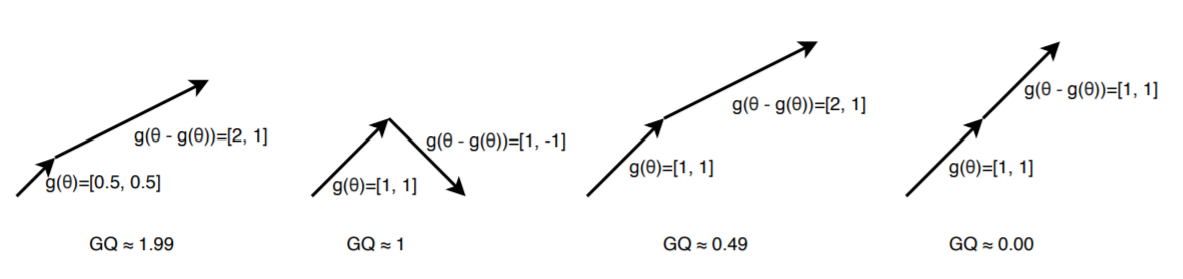
\includegraphics{figures/MetaInit.png}
    \caption{Gradient quotient for different scenarios of initial gradient $g(\theta)$ and gradient after one update $g(\theta - g(\theta))$. A situation where the optimization is locally linear with minimal second order effects (see last example) has a small change between the gradients and thus a small gradient quotient.}
    \label{fig:GQexamples}
\end{figure}

\chapter{Empirical approach to improve our understanding  why variance reduction method fail to  perform well on DNNs}

The main hypothesis we want to test in this paper is \textbf{whether there is a link between the usage of batch-normalization layers in deeper neural networks and the worse results of variance reduced methods}.
A paper from 2019 by Aaron Defazio and Léon Bottou $\textit{On the Ineffectiveness of Variance Reduced Optimization for Deep Learning}$ suggests that applying these techniques on hard non-convex problems generally fails to give good results. However, we note that their analysis does not give any theoretical insights on why this would be the case. Moreover, we see that when testing their assumptions on deeper networks, the architectures they use include batch-normalization layers~\cite{ioffe2015batch}. These layers, because they use averages throughout training as explained in \autoref{eq:BN} break the assumptions that the gradient estimates in \autoref{eq:updateSVRG} for SVRG and \autoref{eq:STORM} for STORM are not unbiased. To test it we compare the results on networks with and without batch-normalization layers.

Another hypothesis we want to test is \textbf{whether initialization methods to better select initial weights for training can help give better results to variance reduced methods in a setting without batch-normalization layers}. Indeed, batch-normalization layers are helping a lot with problems of vanishing and exploding gradients and make it easier to train bigger models, so we think that removing the batch-normalization layers can make training harder but we want to see whether this can be counterbalanced by proper weight initialization.


\chapter{Experiments}
%%%%%%%%%%%%%%%%
\section{Benchmark on shallow Neural Networks}
%%%%%%%%%%%%%%%%
To get insights on how variance reduced methods work we first perform a benchmark on a shallow neural network with different algorithms. We choose to use SVRG, STORM, SGD, Adam and AdaGrad. The first two are the only ones that have a variance reduction effect, SGD and Adam are chosen since they are very popular optimization algorithms and AdaGrad is also benchmarked as it is compared with STORM in its original paper. 

To perform the all subsequent experiments, we need to implement the two variance reduced methods, SVRG and STORM, as there is no official pytorch implementation. The code can be found in the repository of this project.

We compare them on a classification task, recognizing hand-written digits from the MNIST dataset~\cite{lecun2010mnist}. You can see example digits in~\autoref{fig:MNIST_examples}. 

\begin{figure}
    \centering
    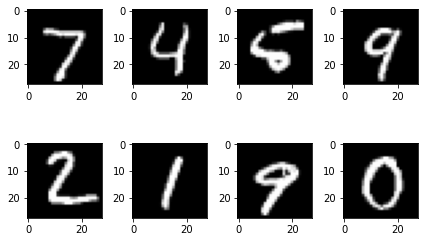
\includegraphics[scale=0.5]{figures/MNIST_example.png}
    \caption{Examples of hand-written digits in the MNIST dataset.}
    \label{fig:MNIST_examples}
\end{figure}

The used architecture is LeNet~\cite{leNet}. The network is presented in \autoref{fig:LeNet}. The Network is composed of two convolutions with a $5 \times 5$ kernel, each followed by an average-pooling layer with a $2 \times 2$ kernel and 3 dense layers at then end. 


\begin{figure}
    \centering
    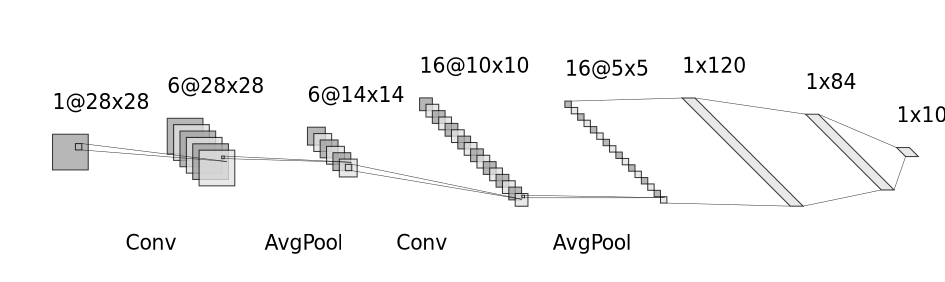
\includegraphics[width=\columnwidth]{midterm presentation/images/LeNet.png}
    \caption{LeNet network used for MNIST}
    \label{fig:LeNet}
\end{figure}

To compare the algorithm we performed a 4-fold cross validation procedure. We did a grid search for the hyperparameters for the algorithms of interest. The considered values are presented in~\autoref{tbl:CVhyperparametersMNIST}. All cross validations were performed for $100$ epochs as this appeared to be long enough for reaching convergence for the algorithms and hyperparameters of interest.  
Note that the hyperparameter $w$ in STORM is not tuned since the original paper already suggests using a value of 0.1 for classifying the MNIST dataset, so we used the proposed value as testing a third hyperparameter would have significantly increased the computational time needed to run the cross-validation.


All experiments are done wit a fixed seed set to 1. We are using a batch size of 32 samples for all runs. The objective we want to minimize is the cross-entropy loss. Given C classes, this loss can be described as:
\begin{equation}\label{eq:CrossEntropyLoss}
    loss(\hat{y}, label) = -log\left(\frac{exp(\hat{y}[label])}{\sum_{c=1}^C exp(\hat{y}[c])}\right)\,,
\end{equation}
where $label$ is the true class of a given datapoint and $\hat{y}$ is a vector with $C$ elements corresponding to the score attributed by the model to the given datapoint for each class.

\begin{table}
    \begin{center}
        \begin{tabular}{||c | c | l||}
             \hline
             Algorithm & Hyperparmeter &  Considered values \\ \hline\hline
ADAM & $\eta$ & $\{10^{-5}, 10^{-4}, 10^{-3}, 0.01, 0.1\}$ \\ \hline
SGD & $\eta$ & $\{10^{-5}, 10^{-4}, 10^{-3}, 0.01, 0.1\}$ \\ \hline
AdaGrad & $\eta$ & $\{10^{-4}, 10^{-3}, 0.01, 0.1\}$ \\ \hline
SVRG & $\eta$ & $\{10^{-5}, 10^{-4}, 10^{-3}, 0.01, 0.1\}$ \\ \hline
STORM & c & $\{0.1, 1, 10, 100, 1000\}$ \\ 
& k & $\{10^{-3}, 0.01, 0.1, 1\}$ \\ \hline

        \end{tabular}
    \end{center}
    \caption{Hyperparameters tested for the 4-Fold cross validation for the different algorithms on LeNet for classification of MNIST hand-written digits.
    }
    \label{tbl:CVhyperparametersMNIST}
\end{table}

To be able to properly compare the results of the different algorithms, we do not compare them in terms of iterations but rather in terms of gradient calculations. This is because SVRG and STORM are doing two gradient calculations per iterations and on top of that SVRG is calculating the whole gradient every m iterations.

For all 5 algorithms, we selected the best hyperparameters based on the best cross-validation error averaged over all 4-folds at the end of the 100 epochs. An example of the results after doing cross-validation for Adam is presented in \autoref{fig:Adamcv}. In this example we see that the best value for the learning rate of Adam for the given task is $10^{-4}$. We see that learning rates with big values are stuck with values of the validation loss which are too high. Values of the learning rate which are too small, although they appear to have significantly less variance, because of the fact that each update only updates the weights by a tiny fraction, do not converge to good results in a reasonable time with our computational capacity. Moreover, small values of the learning rate might lead to situations where the algorithm is stuck in a local minimum of the optimization landscape. 

\begin{figure}
    \centering
    \includegraphics[width=\columnwidth]{midterm presentation/images/AdamCV.png}
    \caption{Cross-validation error during training of Adam optimizer for classification of MNIST dataset on LeNet architecture with gridsearch on selected values of the learning rate $\eta$ (see \autoref{tbl:CVhyperparametersMNIST}). The solid lines represent the average of the loss across the 4 folds (represented by the faded lines) for each iteration.}
    \label{fig:Adamcv}
\end{figure}

After repeating the same method for all algorithms, we present the selected hyperparameters for each algorithm in \autoref{tbl:CVresultsMNIST}.

\begin{table}
    \begin{center}
        \begin{tabular}{||c | c | l||}
             \hline
             Algorithm & Hyperparmeter &  Selected value \\ \hline\hline
ADAM & $\eta$ & $10^{-4}$ \\ \hline
SGD & $\eta$ & $0.1$ \\ \hline
AdaGrad & $\eta$ & $0.1$ \\ \hline
SVRG & $\eta$ & $0.01$ \\ \hline
STORM & c & $100$ \\ 
& k & $0.1$ \\ \hline

        \end{tabular}
    \end{center}
    \caption{Selected hyperparameters after 4-Fold cross validation for the different algorithms on LeNet for classification of MNIST hand-written digits.
    }
    \label{tbl:CVresultsMNIST}
\end{table}

We then compare the 5 algorithms on a test set with the best-tuned hyperparameters to be able to compare them with each other. The results are presented in \autoref{fig:testLossesMnist}. We see that SGD, Adam and AdaGrad are better at first but then the variance reduced methods, SVRG and STORM get better results. The fact that non-variance reduced methods are better at first can be explained by the fact that their iterations require only one gradient computation, so they can advance faster in their optimization.

\begin{figure}
    \centering
    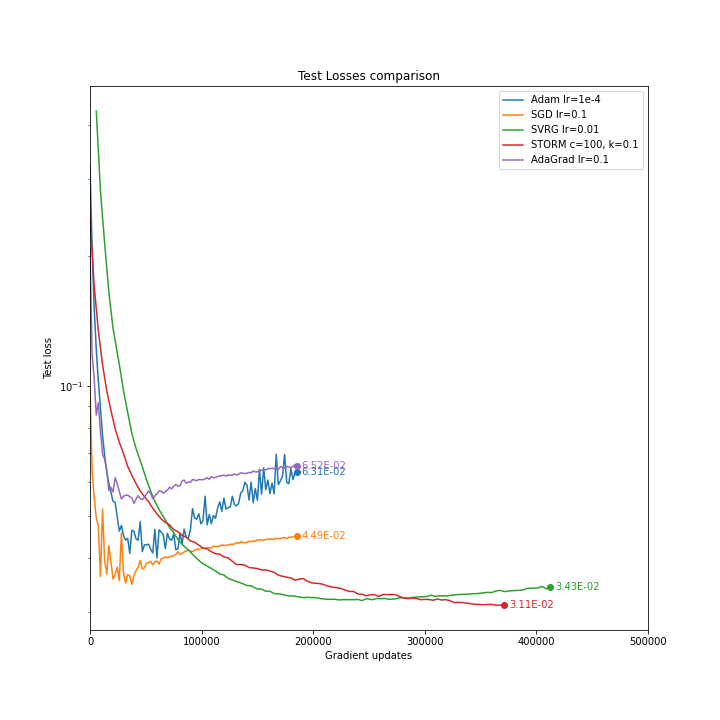
\includegraphics[width=.8\columnwidth]{midterm presentation/images/testLossesMnist.png}
    \caption{Test loss during training of Adam, SGD, SVRG, STORM and AdaGrad with hyperparameters selected after doing a 4-fold cross-validation for classification of the MNIST dataset on a LeNet architecture. The x-axis is in terms of gradient computations. The variance reduced methods are performing better than the others.}
    \label{fig:testLossesMnist}
\end{figure}

We thus see that as expected SVRG and STORM outperform the other stochastic methods in this setup.


%%%%%%%%%%%%%%%%%%%%%%%%
\section{Benchmark on deeper neural networks}
%%%%%%%%%%%%%%%%%%%%%%%%
To check the effect we are hypothesizing we choose a deep neural network with batch-normalization layers and compare Adam, SGD and SVRG. Because of the increased required computational resources we are not able to perform a proper Cross-Validation procedure, rather we select $5\%$ of the training set and use it as a validation set to select the best hyperparameters for each model and then compare them on the test set. Moreover, for the same reason of increased computational time, we are unable to to get meaningful results for STORM as there are more hyperparameters to tune and we don't have insights to properly tune them. However, we think that results found on SVRG could probably also be applied to other variance reduced methods such as STORM.


\subsection{ResNet18 with batch-normalization layers}


The deep neural network we choose to perform our experiments on is ResNet18. This is a network for image recognition introduced in 2015~\cite{he2015deep}. The key idea of this model is that it is constituted of residual learning building blocks with forward connections as presented in~\autoref{fig:building_block_resnet}. These are then put together one after the other as presented in~\autoref{fig:resnet18}. ResNet models with batch-normalization layers have a batch-normalization layer after each convolution layer. If not specifically specified, the ResNet model have batch-normalization layers in all subsequent experiments.

\begin{figure}
    \centering
    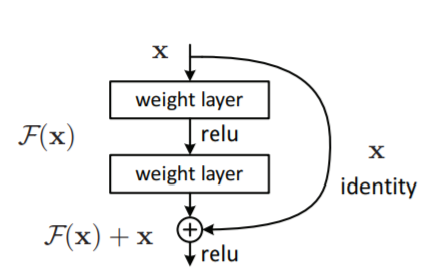
\includegraphics[scale=1]{midterm presentation/images/building_block_ResNet.png}
    \caption{Residual learning: a building block.}
    \label{fig:building_block_resnet}
\end{figure}

\begin{figure}
    \centering
    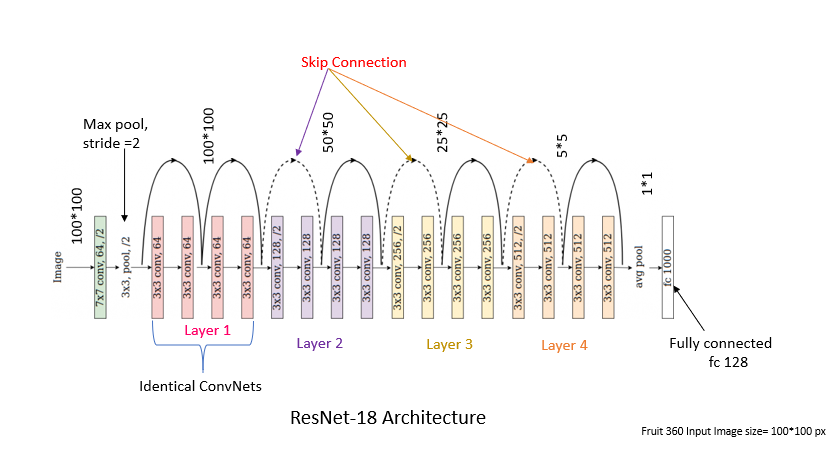
\includegraphics[scale=0.35]{midterm presentation/images/ResNet18.png}
    \caption{ResNet18 architecture with layers and skip connections shown.}
    \label{fig:resnet18}
\end{figure}

The image dataset we are trying to classify is CIFAR-10~\cite{Krizhevsky09learningmultiple}. These images are representing 10 classes: plane, car, bird, cat, deer, dog, frog, horse, ship and truck. A small sample is given in \autoref{fig:CIFAR10_sample}.

\begin{figure}
    \centering
    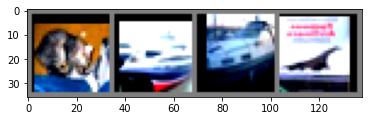
\includegraphics{figures/CIFAR10_sample.png}
    \caption{4 samples from the CIFAR10 image dataset containing images of 10 classes: plane, car, bird, cat, deer, dog, frog, horse, ship and truck. The 4 samples here are cat, ship, ship and plane.}
    \label{fig:CIFAR10_sample}
\end{figure}

We apply the following transforms to these images: we first pad them with 4 pixels on each side, then perform a random square crop of size $32\times32$ and then perform a horizontal flip with probability $0.5$. We finally normalize each channel (reg, green and blue) with the means and standard deviations as calculated from the training set. We then use the Cross-Entropy loss as an objective as described in \autoref{eq:CrossEntropyLoss}. As before, we fix the random seed to 1 and this time we use batches of size 128. We do the training for 200 epochs for each algorithm except for SVRG where we only use 150 epochs. We notice that the best hyperparameters are usually similar or a bit smaller than the ones found in the case of the shallower neural network above. The choices of tested hyperparameters is presented in~\autoref{tbl:ChoicesHyperparametersCIFAR}.

\begin{table}
    \begin{center}
        \begin{tabular}{||c | c | l||}
             \hline
             Algorithm & Hyperparmeter &  Considered values \\ \hline\hline
ADAM & $\eta$ & $\{10^{-5}, 10^{-4}, 10^{-3}\}$ \\ \hline
SGD & $\eta$ & $\{0.005, 0.01, 0.05, 0.1\}$ \\ \hline
SVRG & $\eta$ & $\{0.0005, 0.010, 0.005, 0.01\}$ \\ \hline
%STORM & c & $\{10, 100,\}$ \\ 
%& k & $\{0.01, 0.1\}$ \\ \hline

        \end{tabular}
    \end{center}
    \caption{Hyperparameters tested for validation for the different algorithms on ResNet18 for classification of CIFAR10 images.
    }
    \label{tbl:ChoicesHyperparametersCIFAR}
\end{table}

After performing validation, we choose the best hyperparameters based on the validation loss at the end of training. The best hyperparameters are presented in \autoref{tbl:BestHyperparametersCIFAR}.

\begin{table}
    \begin{center}
        \begin{tabular}{||c | c | l||}
             \hline
             Algorithm & Hyperparmeter &  Selected value \\ \hline\hline
ADAM & $\eta$ & $10^{-4}$ \\ \hline
SGD & $\eta$ & $0.05$ \\ \hline
SVRG & $\eta$ & $0.01$ \\ \hline
%STORM & c & $999$ \\ 
%& k & $999$ \\ \hline

        \end{tabular}
    \end{center}
    \caption{Best hyperparameters after validation for the different algorithms on ResNet18 for classification of CIFAR10 images.
    }
    \label{tbl:BestHyperparametersCIFAR}
\end{table}

We compare the 3 algorithms with the best-tuned hyperparameters on the test set. In \autoref{fig:ResNet18results} we show the test loss during training. 

\begin{figure}
    \centering
    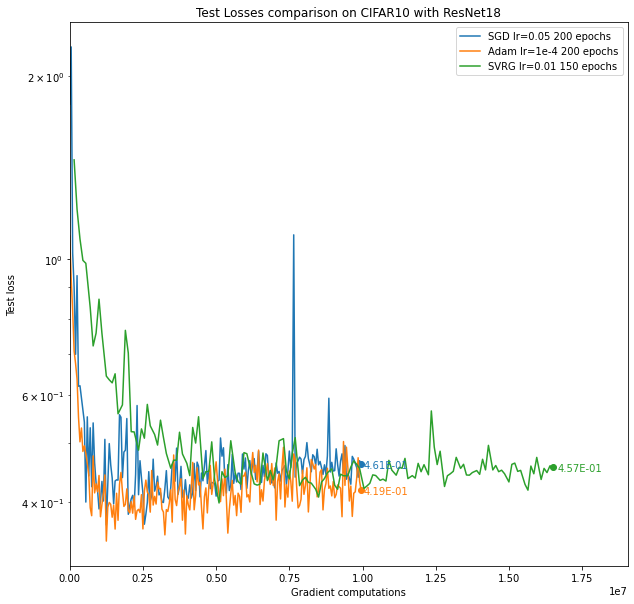
\includegraphics[width=\columnwidth]{figures/ResNet18Results.png}
    \caption{Test loss during training of SGD, Adam and SVRG with hyperparameters selected on the validation set for classification of the CIFAR10 dataset on a ResNet18 architecture. The x-axis is in terms of gradient computations. SVRG does not have better results in this setting.}
    \label{fig:ResNet18results}
\end{figure}

We see that in this setting the variance reduced method, SVRG is not outperforming the other methods as in the case of the shallow neural network. 

\subsection{ResNet18 without batch-normalization layers}

To test our hypothesis we do the same analysis on the same network, ResNet18, except that this time we remove the batch-normalization layers. We do the same validation process with the same values (see \autoref{tbl:ChoicesHyperparametersCIFAR}). One think that we notice during this phase is that finding the correct hyperparameters becomes even more crucial in this scenario, as there are some choices for which the values become irrelevant. For example, we started getting $NaN$ results for high learning rates of SGD. This might be due to problems of exploding gradients but we do not explore the exact reasons further as other choices of hyperparameters yield good results. However, it is important to note that removing batch-normalization layers can make some choices of hyperparameters completely irrelevant, although they were still getting acceptable results, although not the best, in a setting with a network with batch-normalization layers.

The selected hyperparameters for each algorithm are presented in \autoref{tbl:BestHyperparametersResNet18noBN}.

\begin{table}
    \begin{center}
        \begin{tabular}{||c | c | l||}
             \hline
             Algorithm & Hyperparmeter &  Selected value \\ \hline\hline
ADAM & $\eta$ & $10^{-5}$ \\ \hline
SGD & $\eta$ & $0.01$ \\ \hline
SVRG & $\eta$ & $0.005$ \\ \hline


        \end{tabular}
    \end{center}
    \caption{Best hyperparameters after validation for the different algorithms on ResNet18 for classification of CIFAR10 images.
    }
    \label{tbl:BestHyperparametersResNet18noBN}
\end{table}

We notice that the choices of the best hyperparameters are always a little bit smaller than in the setting with a network with batch-normalization layers when we compare with the choices in \autoref{tbl:BestHyperparametersCIFAR}.

The results on the test set are presented in \autoref{fig:ResNet18noBNresults}.

\begin{figure}
    \centering
    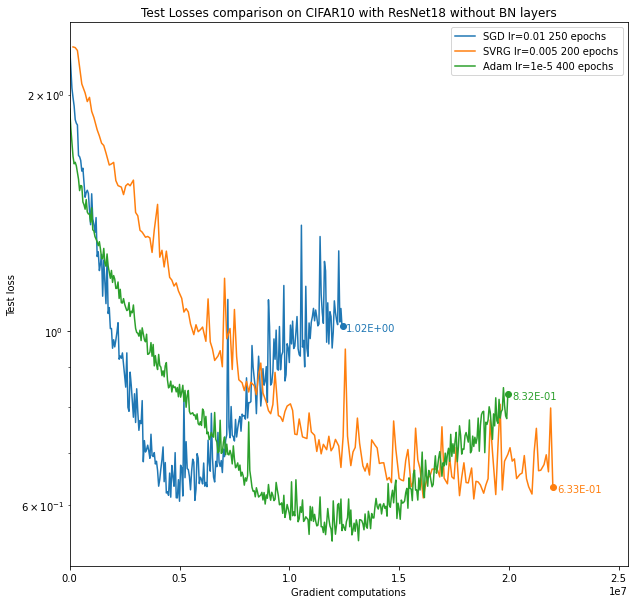
\includegraphics[width=\columnwidth]{figures/ResNet18noBNResults.png}
    \caption{Test loss during training of SGD, Adam and SVRG with hyperparameters selected on the validation set for classification of the CIFAR10 dataset on a ResNet18 architecture without batch-normalization layers. The x-axis is in terms of gradient computations.}
    \label{fig:ResNet18noBNresults}
\end{figure}

In this setting we see that SVRG seems to get to better results that the other methods which are affected a lot by the removal of the batch-normalization layers. SVRG seems to be less negatively affected by the removal of the batch-normalization layers. We notice that the best test loss in this setting is not as good as in the setting when we do have batch-normalization layers.

\subsection{ResNet101 with batch-normalization layers}

To test our hypothesis even further we do a similar approach on a deeper neural network. To do so we choose the ResNet101 architecture. This network is similar to ResNet18 except that is has more layers stacked one after the other. A figure from the original paper presenting the ResNet architecture~\cite{he2015deep} summarizes the differences and is presented in \autoref{fig:ResNetarchitectures}.

\begin{figure}
    \centering
    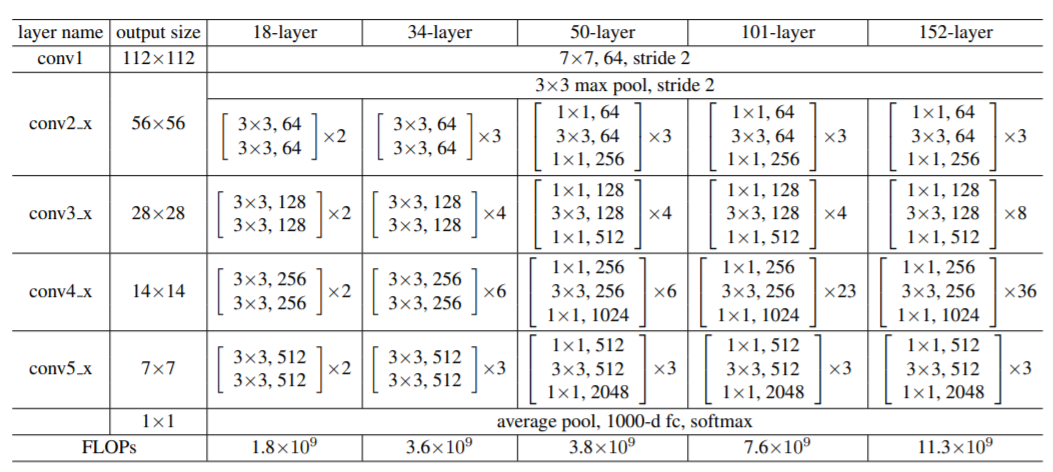
\includegraphics{figures/ResNetArchitectures.png}
    \caption{Different variants of the ResNet architecture presented in the original paper. Building blocks are shown in brackets, with the numbers of blocks stacked. Downsampling is performed by conv$3\_1$, conv$4\_1$, and conv$5\_1$ with a stride of 2.}
    \label{fig:ResNetarchitectures}
\end{figure}

For this new architecture we perform a similar classification task but on a bigger dataset with more classes, CIFAR100~\cite{Krizhevsky09learningmultiple}. Some images from this dataset are presented in \autoref{fig:CIFAR100_sample}.

\begin{figure}
    \centering
    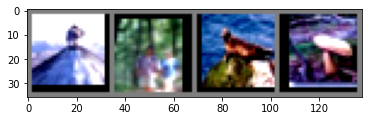
\includegraphics{figures/CIFAR100_sample.png}
    \caption{4 samples from the CIFAR100 image dataset containing images of 100 classes. The 4 samples here are mountain, forest, seal and mushroom.}
    \label{fig:CIFAR100_sample}
\end{figure}

For this task we perform on the images the same transformations and preprocessing as with CIFAR10. We first pad them with 4 pixels on each side, then perform a random square crop of size 32×32 and then perform a horizontal flip with probability 0.5 and finally we normalize each channel (reg, green and blue) with the means and standard deviations as calculated from the training set. Then we repeat the same steps as we did for ResNet18. We first use a validation set of $5\%$ to select the best hyperparameters and then compare on the test set the cross entropy loss with the best tuned hyperparameter for Adam, SGD and SVRG. The hyperparameters we checked in the validation phase are presented in \autoref{tbl:ChoicesHyperparametersCIFAR100}. We notice that we usually need similar learning rates than the smaller ResNet18 network, as shown in \autoref{tbl:BestHyperparametersCIFAR100}.

\begin{table}
    \begin{center}
        \begin{tabular}{||c | c | l||}
             \hline
             Algorithm & Hyperparmeter &  Considered values \\ \hline\hline
ADAM & $\eta$ & $\{10^{-6}, 10^{-5}, 10^{-4}\}$ \\ \hline
SGD & $\eta$ & $\{0.005, 0.01, 0.05\}$ \\ \hline
SVRG & $\eta$ & $\{0.0005, 0.010, 0.005\}$ \\ \hline
        \end{tabular}
    \end{center}
    \caption{Hyperparameters tested for validation for the different algorithms on ResNet101 for classification of CIFAR100 images.
    }
    \label{tbl:ChoicesHyperparametersCIFAR100}
\end{table}

\begin{table}
    \begin{center}
        \begin{tabular}{||c | c | l||}
             \hline
             Algorithm & Hyperparmeter &  Selected value \\ \hline\hline
ADAM & $\eta$ & $10^{-4}$ \\ \hline
SGD & $\eta$ & $0.05$ \\ \hline
SVRG & $\eta$ & $0.005$ \\ \hline

        \end{tabular}
    \end{center}
    \caption{Best hyperparameters after validation for the different algorithms on ResNet101 for classification of CIFAR100 images.
    }
    \label{tbl:BestHyperparametersCIFAR100}
\end{table}

The results of the test set are presented in \autoref{fig:ResNet101results}. It appears that SVRG with best-tuned hyperparameters has results that are consistently worse than both Adam and SGD at any point during training. However, we can note that the difference is not extreme between the variance reduced method and the others.

\begin{figure}
    \centering
    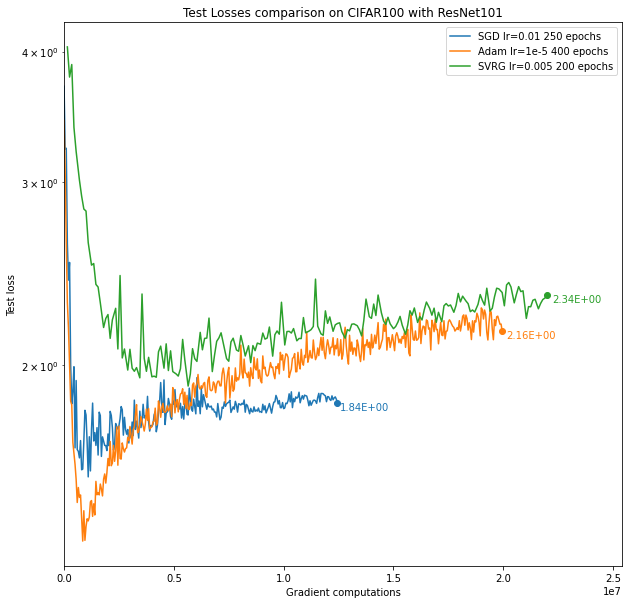
\includegraphics[width=\columnwidth]{figures/ResNet101Results.png}
    \caption{Test loss during training of SGD, Adam and SVRG with hyperparameters selected on the validation set for classification of the CIFAR100 dataset on a ResNet101 architecture with batch-normalization layers. The x-axis is in terms of gradient computations.}
    \label{fig:ResNet101results}
\end{figure}





\subsection{ResNet101 without batch-normalization layers}\label{seq:ResNet101noBN}

We perform the exact same setup as what we did with above with ResNet101 and CIFAR100, except that this time we remove the batch-normalization layers to test once more the hypothesis we formulated at the beginning. We check the same hyperparameters on the validation set (see \autoref{tbl:ChoicesHyperparametersCIFAR100}) and the best learning rate for each algorithm is presented in \autoref{tbl:BestHyperparametersCIFAR100noBN}.

\begin{table}
    \begin{center}
        \begin{tabular}{||c | c | l||}
             \hline
             Algorithm & Hyperparmeter &  Selected value \\ \hline\hline
ADAM & $\eta$ & $10^{-4}$ \\ \hline
SGD & $\eta$ & $0.005$ \\ \hline
SVRG & $\eta$ & $0.005$ \\ \hline

        \end{tabular}
    \end{center}
    \caption{Hyperparameters tested for validation for the different algorithms on ResNet101 without batch-normalization layers for classification of CIFAR100 images.
    }
    \label{tbl:BestHyperparametersCIFAR100noBN}
\end{table}

The results on the test set are presented in \autoref{fig:ResNet101noBNresults}. We see that in this setup SVRG seems to have similar and sometimes better results than the other algorithms, which was not the case with ResNet101 with batch-normalization layers. 

\begin{figure}
    \centering
    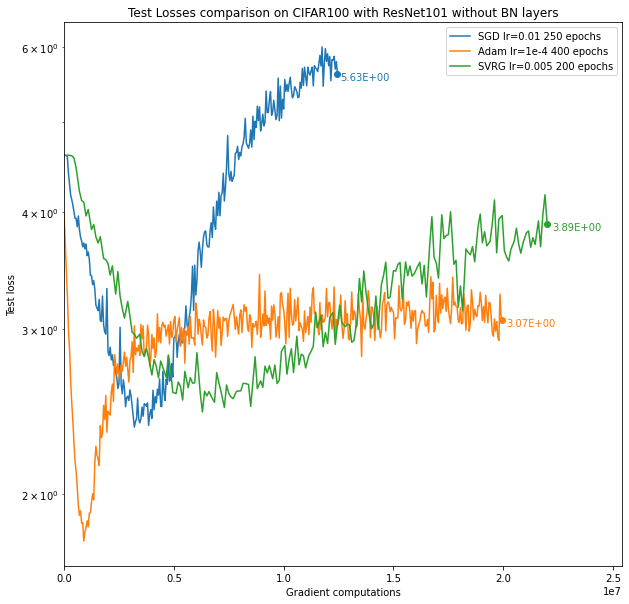
\includegraphics[width=\columnwidth]{figures/ResNet101noBNResults.png}
    \caption{Test loss during training of SGD, Adam and SVRG with hyperparameters selected on the validation set for classification of the CIFAR100 dataset on a ResNet101 architecture without batch-normalization layers. The x-axis is in terms of gradient computations.}
    \label{fig:ResNet101noBNresults}
\end{figure}

\section{Effects of MetaInit}
In the previous experiments we see that it seems that SVRG gets comparable and even sometimes better results than Adam and SGD in the setup without batch-normalization. However, we note that all results of all the 3 algorithms worsen a little bit relative to their respective results in the case when we use batch-normalization layers. This might be due to effects of the batch-normalization layers which help reach better convergence that are lost when removing these layers. To counter this we think that using better initialization methods than the ones used by default in Pytorch could get better results in the setup without batch-normalization layers. For now, all experiments we did used the default initialization implemented by Pytorch as of January 2021, some examples are given below. \autoref{eq:initLinearLayers} for Linear layers with $in\_feature$ input features of the layer and \autoref{eq:initConv2dLayers} for 2 dimensional convolutional layers with $C\_in$ input channels and $kernel\_size$ is a tuple containing the size of the kernel in the 2 dimensions and $*$ is the valid 2D cross-correlation operator. 

\begin{equation}\label{eq:initLinearLayers}
    \mathcal{U}(-\sqrt{k}, \sqrt{k}) \text{, where } k = \frac{1}{in\_features}
\end{equation}

\begin{equation}\label{eq:initConv2dLayers}
    \mathcal{U}(-\sqrt{k}, \sqrt{k}) \text{, where }
    k = \frac{1}{C\_in * \prod_{i=0}^{1}kernel\_size[i]} 
\end{equation}

To test the effects of weight algorithm MetaInit described previously, we run an experiment with SVRG on ResNet101 with a classification task of the CIFAR100 dataset with the same hyperparameters as the ones described in \autoref{seq:ResNet101noBN}. We use the same learning rate of $0.005$ and run the training of SVRG for 200 epochs. We run the Gradient descent part of the MetaInit algorithm for 200 epochs with a learning rate of $0.1$, momentum of $0.9$ and $\epsilon = 10^{-5}$.  

The results on the test set between a run using MetaInit and one not using it are compared in \autoref{fig:MetaInitresults}. We see that the experiment with MetaInit doesn't seem to outperform extremely the algorithm without batch-normalization layers. This probably suggests that the default weight initialization used by Pytorch is already performing well on such an architecture and that MetaInit does not seem to add a lot. 

\begin{figure}
    \centering
    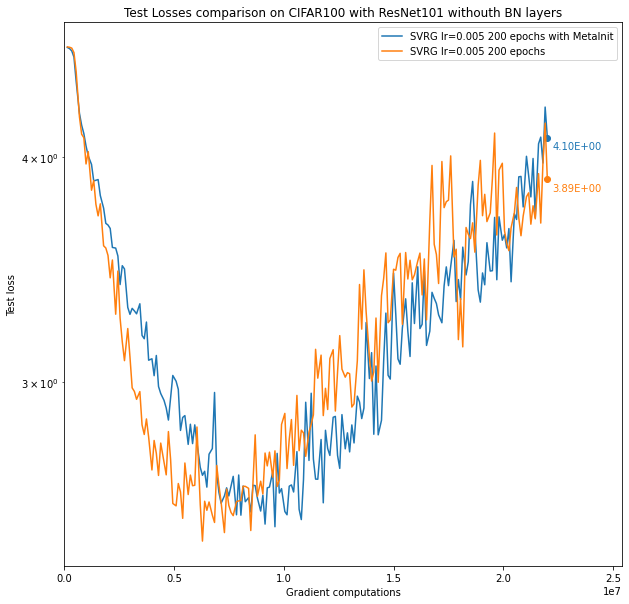
\includegraphics[width=\columnwidth]{figures/MetaInitresults.png}
    \caption{SVRG on ResNet100 for classification of CIFAR100. Comparison of two experiments with the same hyperparameters and MetaInit applied to one of the experiments.}
    \label{fig:MetaInitresults}
\end{figure}

%%%%%%%%%%%%%%%%%%%%
\chapter{Conclusion}
%%%%%%%%%%%%%%%%%%%%

After the various experiments, we see that stochastic variance reduced gradient methods are performing better than Adam and SGD on smaller architectures such as LeNet for classification of MNIST and we see that when applied on common Deep Neural Networks with batch-normalization layers the variance reduced method SVRG is outperformed by Adam and SGD.
Because the batch-normalization layers are breaking the assumption of unbiasedness of the updates of SVRG, we test the same setups with architectures where batch-normalization layers have been removed and note that in this case SVRG gets comparable and sometimes better results than Adam and SGD. 

However, when doing this we note two things. First, searching for good hyperparameters is harder when batch-normalization layers are removed as we get scenarios with DNNs that get irrelevant results in some hyperparameter setups. 
Second, we note that the best results reached with all three algorithms (SGD, Adam and SVRG) on the network are not as good as the best results on the same network with batch-normalization layers.

To try to tackle this problem we try using a weight initialization method, MetaInit. However, this doesn't seem to help significantly. 

In summary, we seem to observe that SVRG is not disadvantaged as much as the other algorithms when removing batch-normalization layers from common DNNs but there are other unexplained phenomena that make the results somehow worse.

We think that future work can be done in order to perform better hyperparameter selection with ResNet18 and ResNet101 by performing a proper cross-validation procedure. Moreover, we think that doing this cross-validation procedure together with MetaInit can help as the better choices of initial weights can allow for more favorable learning rates that were not possible when the batch-normalization layers are removed. Finally we think that experiments should be tested with more DNNs and data-sets and random seeds in order to get more conclusive result. 

\makeacks


\cleardoublepage
\phantomsection
\addcontentsline{toc}{chapter}{Bibliography}
\printbibliography

\end{document}